\section{Experiments And Results}
\label{sec:evaluation}
As described in section \ref{sec:visual-aspects} \emph{Deep Dream} works by selecting layers and neurons that should be activated more.
In order to select good layers for the dreaming, we let each layer be dreamed onto an image to handpick the layers that offer interesting features.
Some of these results can be seen in section \ref{sec:withoutguide}.

To get a more granular control of the intensified features, one can use a \textit{guide image}.
A \textit{guided dream}, described in section \ref{guided-dreaming}, will select neurons based on the \textit{guide image} in that layer.
The results are presented in section \ref{sec:withguide}.

All images are created using the default parameters given by the \textit{Google Deep Dream} code.
These are 4 \textit{octaves} with a scale factor of 1.4, 10 iterations, a step size of 1.5 and a jitter of 32 pixels.
Experiments with different parameters can be found in section \ref{sec:varying-parameters}.


\subsection{Performance Considerations}
\label{sec:performance}
The runtime of the \textit{Deep Dream} depends mostly on the size of the input image and the layer amount.
Using an image of $\approx$600x430 pixels, 30 layers, 10 iterations and 4 \textit{octaves} can already take around 45 minutes and uses up to 14GB of RAM\footnote{executed with a single thread on an i7-5930k@3,5GHz and 32GB RAM}.
We also implemented the \textit{bilateral} filter which will be applied after every step or after every octave.\cite{bilateral}
This also slows down the runtime because the application of the filter takes a few seconds to compute.

\newpage
\subsection{A closer look into the layers}
\label{sec:withoutguide}

As mentioned in section \ref{sec:data}, the analyzed model contains 50 layers, so we will not be showing the dreaming results for each one, but rather a selection that we deemed satisfactory.
Throughout these layers one can find all kinds of features varying from different colors, textures to small parts of objects.
Looking at figure \ref{fig:14-landscape} one can see that the recognizable features within a layer are not limited to a particular one and includes transitions between the different textures.
These transitions seem to distinguish pixelated regions from very sharp ones.
But it can also result in a transition from smooth curves to very straight lines, see figure \ref{fig:16-landscape}.

\begin{figure}[H]
	\minipage{0.32\textwidth}
	\centering
	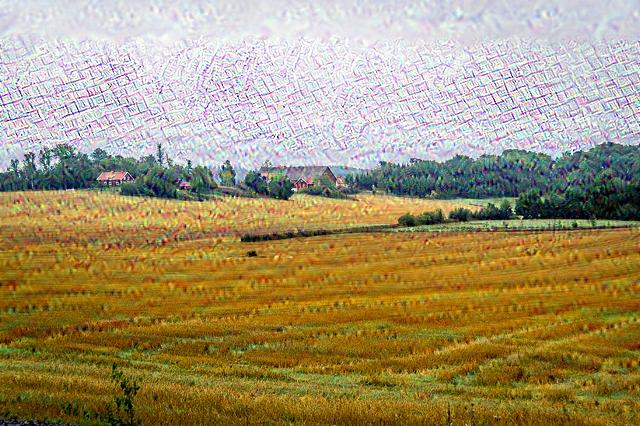
\includegraphics[width=1\linewidth]{img/14_alpsted-landscape_res3a_branch2b.jpg}
	\caption{Dream with layer 14 \emph{res3a\_branch2b}.}
	\label{fig:14-landscape}
	\endminipage\hfill
	\minipage{0.32\textwidth}
	\centering
	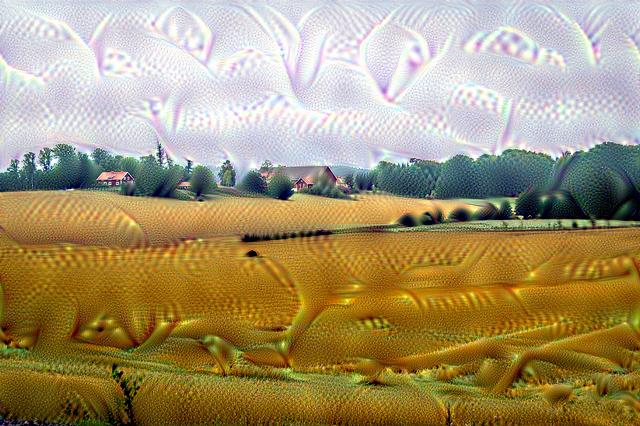
\includegraphics[width=1\linewidth]{img/16_alpsted-landscape_res3b_branch2a.jpg}
	\caption{Dream with layer 16 \emph{res3b\_branch2a}.}
	\label{fig:16-landscape}
	\endminipage\hfill
		\minipage{0.32\textwidth}
	\centering
	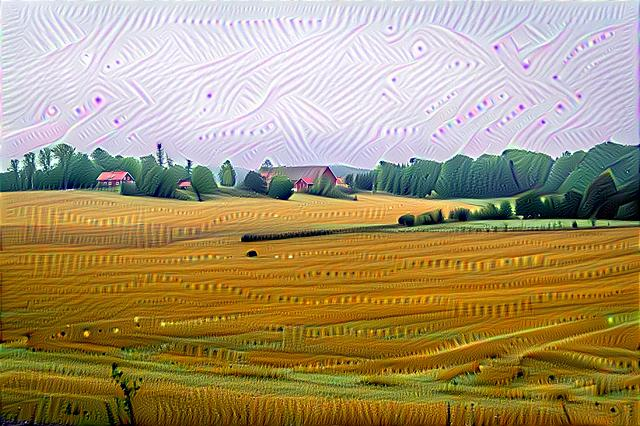
\includegraphics[width=1\linewidth]{img/alpsted-landscape_res3a_branch1.jpg}
	\caption{Dream with layer 12 \emph{res3a\_branch1}.}
	\label{fig:layer-artistic}
	\endminipage\hfill
\end{figure}

Another interesting find is layer 12 depicted in figure \ref{fig:layer-artistic}.
If one ignores the lines and purple tint it looks like an artistic style filter was applied.
This supports DiPaolo's findings, mentioned in section \ref{sec:previous-work}, that by using the right combination of neurons \textit{Deep Dream} can be used to modify pictures such that they look like paintings.

\begin{figure}[H]
	\centering
	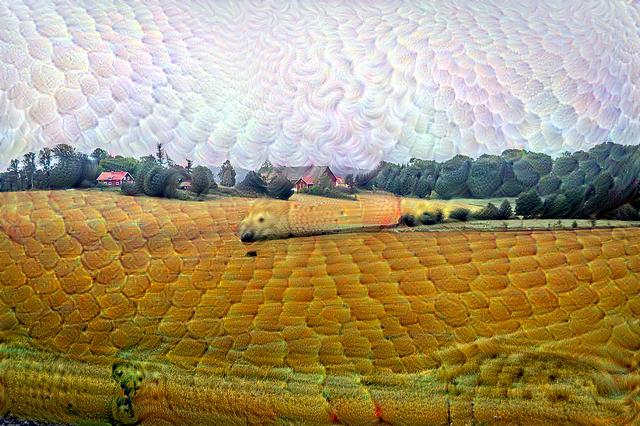
\includegraphics[width=0.7\linewidth]{img/alpsted-landscape_res4f_branch2a.jpg}
	\caption{Dream with layer 41 \emph{res4f\_branch2a}: Snake scales with a snake head in the lower left.}
	\label{fig:layer-snake}
\end{figure}

Going further up in the layers we found one layer of particular interest, depicted in figure \ref{fig:layer-snake}.
It visualizes four distinct things at once which makes it unique.
There is a snake's head in the lower left part of the image as well as to the right of the very left house.
The field and large parts of the sky were transformed to look like snake scales.
Apart from these two already distinctive objects the center seems to contain the right part of a dog's face and above it, the sky looks more like dog fur.

An additional applied change that can be observed in almost all layers is a slight purple to rainbowish tint that gets applied to the image, especially around the newly added features, as visible within the lines in figure \ref{fig:layer-artistic} and in the sky of figure \ref{fig:layer-snake}.




\subsection{Varying Parameters}
\label{sec:varying-parameters}
In section \ref{sec:optimizations}, we mentioned the varying parameters that can be used to optimize the results, hence we will experiment with them here.

To show the effect of more iterations, we have increased them by a factor of ten to 100 in total.
This results in images, where few of the original aspects are still visible, but the learned features dominate the visual appearance.
This can be very well seen in figure \ref{fig:baum}.
Here branches of a tree prevail the sky and the field was replaced by shrubs.
The houses have been eradicated by trees.

\begin{figure}[H]
	\centering
	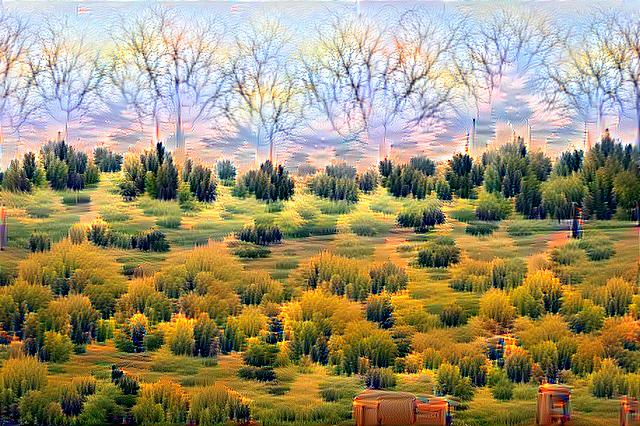
\includegraphics[width=0.7\linewidth]{img/baum}
	\caption{100 iterations dream with layer 37 \emph{res4d\_branch2c} onto the field}
	\label{fig:baum}
\end{figure}

Sometimes higher iterations are not sufficient to fully transform every aspect of an image.
This can be seen in figure \ref{fig:houses1} at the houses on the left, that remain almost untouched.
When we also increase the step size from 1.4 to 2.0 we were able to modify the image beyond recognition, see figure \ref{fig:houses2}.
By increasing both parameters, we were able to clearly visualize the learned features within the layer.


\begin{figure}[H]
	\minipage{0.49\textwidth}
	\centering
	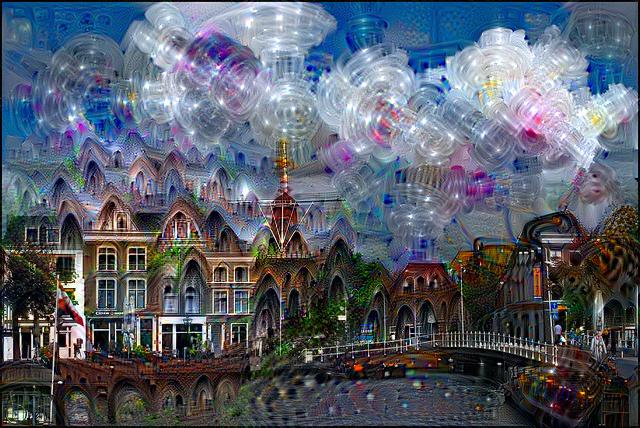
\includegraphics[width=1\linewidth]{img/houses1.jpg}
	\caption{Dream with layer 43 \emph{res4f\_branch2c} onto the Beestenmarkt with a \emph{step size} of 1.4.}
	\label{fig:houses1}
	\endminipage\hfill
	\minipage{0.49\textwidth}
	\centering
	
\includegraphics[width=1\linewidth]{img/houses2.jpg}
	\caption{Dream with layer 43 \emph{res4f\_branch2c} onto the Beestenmarkt with a \emph{step size} of 2.}
	\label{fig:houses2}
	\endminipage\hfill
\end{figure}

\subsection{Bilateral Filter}
\label{sec:bilateral}

As mentioned in section \ref{sec:optimizations}, the \emph{bilateral} filter is used for smoothing out sharp edges.
Because feature transitions in dreamed images are sometimes harsh we chose to use this filter.

The default parameters are used, except the  iteration amount has been increased to 100.
We decided to apply the filter at two different stages of the dreaming process.
In figure \ref{fig:bilateral1} you can see a dream where the filter is applied after every iteration, hence 400 times.
This is very clearly visible in the clouds that have turned completely flat and don't give the \emph{Deep Dream} anything to act upon. 
We also assume, that some added features got smoothed out too quickly.


\begin{figure}[H]
	\minipage{0.49\textwidth}
	\centering
	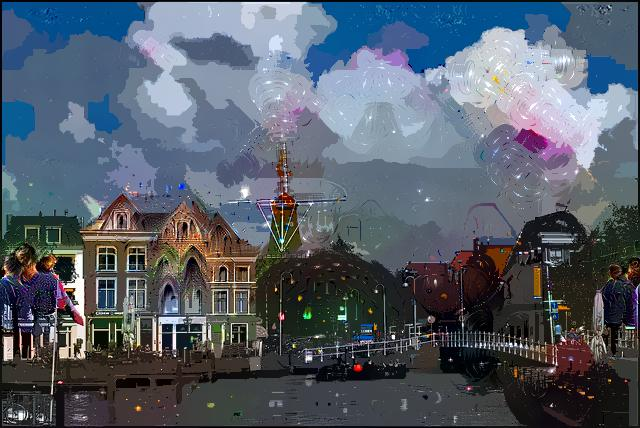
\includegraphics[width=1\linewidth]{img/bilateral1.jpg}
	\caption{Dream with layer 43 \emph{res4f\_branch2c} onto the Beestenmarkt with 100 iterations and \emph{bilateral} filter}
	\label{fig:bilateral1}
	\endminipage\hfill
	\minipage{0.49\textwidth}
	\centering
	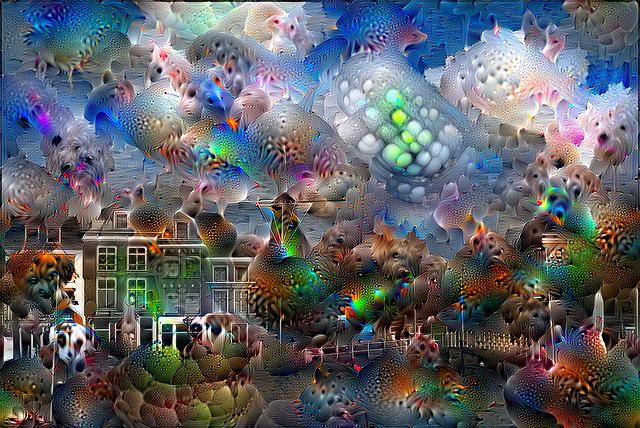
\includegraphics[width=1\linewidth]{img/beestenmarkt_res5a_branch1_bilateral.jpg}
	\caption{Dream with layer 44 \emph{res5a\_branch1} onto the Beestenmarkt with 100 iterations and \emph{bilateral} filter.}
	\label{fig:bilateral2}
	\endminipage\hfill
\end{figure}
\newpage

The generated image underlines the multitude of recognized objects embedded into only a single layer.
We used the same layer as in figure \ref{fig:houses2}, which previously generated houses.
In the \emph{bilateral} run the added houses are barely visible.
However humans seem to appear in left and right lower corner.
This is surprising, because in the dream layer collection we created, no humans were found.

Applying the \emph{bilateral} filter after every octave meaning only 4 times in total obviously affects the outcome less stronger, see figure \ref{fig:bilateral2}.
The dreaming works very well and the result is less sharp than the previous dreams.
We consider this beneficial because it enables smoother dreams that look more naturally painted.





\subsection{Guided Dream}
\label{sec:withguide}
Following up on section \ref{guided-dreaming}, we want to highlight the possibilities opened up through \textit{guided dreaming}.
We decided to choose a picture of puppies, because the \emph{ImageNet} dataset contains a large amounts of varying dog breeds.
Because we let each layer be dreamed onto an image, we could select one that seems to resemble dogs or animals.
We ended up choosing layer 33 \emph{res4c\_2b}.
As one can see, by using only 50 iterations in combination with a \textit{guide image}, features of dogs overshadow the original image.

We also evaluated the effect of an increased \emph{step size}, but omitted the results because the visual difference was not nearly as clear as in the previous section.

\begin{figure}[H]
	\minipage[t]{0.40\textwidth}
	\centering
	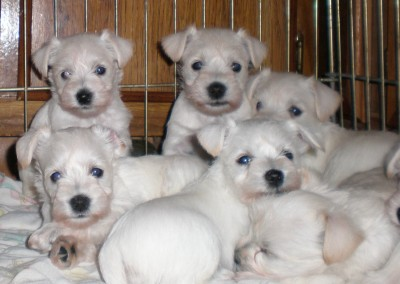
\includegraphics[width=1\linewidth]{img/guide.jpg}
	\caption{Guide image\cite{imgpuppies}}
	\label{fig:guide}
	\endminipage\hfill
	\minipage[t]{0.59\textwidth}
	\centering
	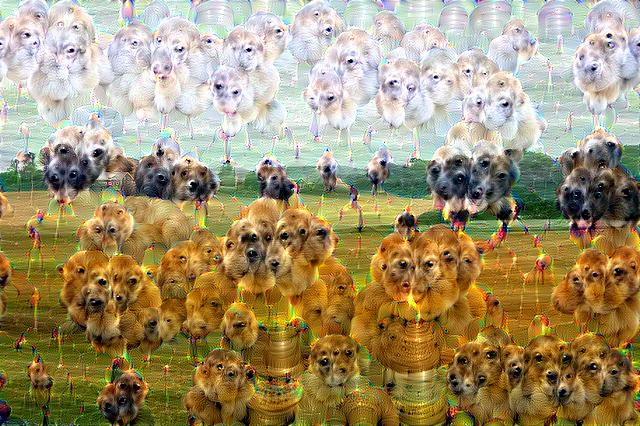
\includegraphics[width=1\linewidth]{img/guide_dream.jpg}
	\caption{Dream with layer 33 \emph{res4c\_branch2b} using the \emph{guide image}.}
	\label{fig:guide_dream}
	\endminipage\hfill
\end{figure}



\subsection{Repeating Features}
\label{sec:repeating-features}

Within the different layers we found some to behave quite similar.
Previously we presented layers that differ from each other in form, size and shape.
Here we present layers that seem to have learned almost the same features.
To show the behavior in the clearest way possible we applied dreaming onto the same random generated noise.
As one can see in the figures \ref{fig:rotated_feature_1} and \ref{fig:rotated_feature_2}, the created images look almost the same, the only real difference is the orientation.
It looks like the enhanced features were simply rotated.

\begin{figure}[H]
	\minipage{0.49\textwidth}
	\centering
	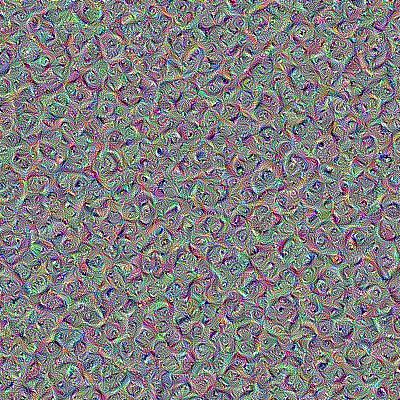
\includegraphics[width=0.9\linewidth]{img/rotated_feature_1.jpg}
	\caption{Dream with layer 7 \emph{res2c\_branch2b} onto random noise}
	\label{fig:rotated_feature_1}
	\endminipage\hfill
	\minipage{0.49\textwidth}
	\centering
	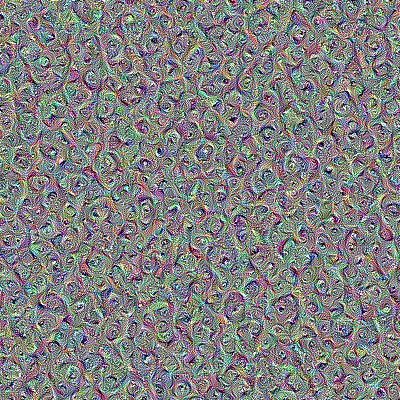
\includegraphics[width=0.9\linewidth]{img/rotated_feature_2.jpg}
	\caption{Dream with layer 8 \emph{res2c\_branch2c} onto random noise}
	\label{fig:rotated_feature_2}
	\endminipage\hfill
\end{figure}

